%==============================================================================
%  mathematics.tex : MATHEMATICAL BACKGROUND
%==============================================================================
% -- NEW COMMANDS FOR NAVIER STOKES EQUATIONS
\newcommand{\CROSS}[2]{ \vec{#1} \times \vec{#2} }
\newcommand{\DOT}[2]{\vec{#1} \bullet \vec{#2}}
\newcommand{\GRAD}[1]{\nabla #1}
\newcommand{\LAP}[1]{\nabla^2 #1}
\newcommand{\CORIOLIS}[1]{2\CROSS{\Omega}{#1}}
\newcommand{\CENTRIFUGAL}[1]{\vec{\Omega} \times (\CROSS{\Omega}{#1})}


% -- TABLE SETTINGS 
\renewcommand{\arraystretch}{1.05} % -- ADD PADDING TO LaTex TABLES


% ----------------- DECLARE CHAPTER TITLE ----------------- %
\chapter{Mathematical background}
\label{math_chapter}
%------------------------------------------------------------------------------
%%%%%%%%%%%%%%%%%%%%%%%%%%%%
% NAVIER - STOKES EQUATION
%%%%%%%%%%%%%%%%%%%%%%%%%%%%%
\section{Navier-Stokes Equations}
The Navier-Stokes equations  (honoring Claude-Louis Navier and George Gabriel Stokes) are a set of partial differential equations that define the motion of a parcel of fluid. 
Solutions to these equations define the velocity field at a particular time and point in space. The equations are derived from applying Newton's second law to a fluid parcel, see \citep{kundu_cohen} for a derivation. These equations are important in any situation that has fluid flow, such as modeling currents in the ocean or the dynamics of a aircraft. These equations were written down in the 19th century and are still relevant today in a practical and academic sense. In a rotating reference frame the Navier-Stokes equations are defined in vector notation as : 

% -- INCOMPRESSIBLE NAVIER STOKES EQUATION
\begin{equation} 
	 \rho(\dtp{\vec{V}} +\DOT{\vec{V}}{\nabla \vec{V}})= -\GRAD{P}  -\rho(\CORIOLIS{V}) - \rho\vec{g_n} -\rho\CENTRIFUGAL{R}+  \mu \LAP{\vec{V}} 
\end{equation} 


% -- DEFINITION OF TERMS
\begin{table}[H]
	\centering
		\caption[Navier-Stokes equation variables]{Definition of variables in the Navier-Stokes equations.} \vspace{6pt}
	\label{table:nse_vars}
	\begin{tabular}{c c}
	\hline  \hline
	\textbf{Term} 				        & \textbf{Description}      							      		    \\ [1ex]  \hline  
	$\vec{V}$		                                    & Velocity vector : $\vec{V}=u\hat{x} + v\hat{y} + w\hat{z}$                        \\ 
	$\vec{R}$					        & Displacement vector : $\vec{R} = x\hat{x} + y\hat{y} + z\hat{z}$            \\ 
	$\rho $                    		                 &  Fluid density   		 								    \\ 
	$\dtp{\vec{V}}$    		                 & Acceleration of fluid parcel  						   		    \\ 
	$\DOT{\vec{V}}{\nabla \vec{V}}$       &  Convective acceleration                 				      		             \\ 
	$\GRAD{P}  $                                       & Pressure gradient          					                       		    \\ 
	$\CORIOLIS{V})$                                 &  Coriolis acceleration            			   		            		    \\ 
	$\CENTRIFUGAL{r}$                          &  Centrifugal acceleration   		  				   		    \\ 
	$\mu \LAP{\vec{V}}$   	 	        &  Shear stress    				        			             		    \\ 
	$\vec{g_n}$       			        & Newtonian gravitational acceleration   						    \\ 
	$\Omega$       				        & Rotation rate of Earth					    		                       \\ [1ex] 
	\hline
	\end{tabular}		
\end{table}

% -- DISCUSSION OF CORIOLIS AND  CENTRIFUGAL ACCELERATIONS
The reference frame is oriented so positive $x$ is to the east, positive $y$ is to the north, and positive $z$ is upward and pointing away from the surface of the Earth.
Two terms in this expression arise because observations are made from a  rotating (non-inertial) reference frame, the Coriolis acceleration (honoring Gaspard-Gustave Coriolis) 
($\CORIOLIS{V}$) and the  centrifugal acceleration (Latin for "center fleeing")  ($ \CENTRIFUGAL{R}$). 
Keep in mind that these are not "real"  accelerations in the sense that we can not name a force that is causing them, it is more appropriate to think of these as apparent accelerations that 
arise due to our frame of reference. 
The centrifugal acceleration is an apparent acceleration that is evoked in a non-inertial (accelerating) reference frame, which is opposite to the
 centripetal (center seeking) acceleration. To simplify the Navier-Stokes equation the centrifugal acceleration vector can be added to gravitational 
 acceleration vector to define an affective gravitational acceleration ($-\vec{g}=-\vec{g_n} -\CENTRIFUGAL{R}$). The Coriolis acceleration gives rise to an apparent 
 deflection of an object when it is moving; this deflection is clockwise in the northern hemisphere and counter-clockwise in the southern hemisphere. 
The components of the Coriolis acceleration are defined as : 
 
 % -- REWRITING CORIOLIS AS = fV
 \begin{align}
 	\CORIOLIS{V} &= 2\Omega \SIN{\phi} v \hat{x} - 2\Omega \SIN{\phi} u \hat{y}\\
	&= -fv\hat{x} + fu \hat{y}
 \end{align}
where $f=2\Omega \SIN{\phi}$ is the Coriolis frequency, $\Omega=\frac{2\pi}{\text{day}}$ is the rotational frequency of Earth and $\phi$ is latitude. The Coriolis period
is given by $T=\frac{2 \pi}{f}$. In Duluth, Minnesota (46.7$^{\circ}$), located at the tip of Lake Superior's western arm, $f \approx 1.1 *10^{-4} \text{s$^{-1}$}$ and the Coriolis period 
is $T \approx 16 \text{\ hrs}$. The physical meaning to the Coriolis frequency will be discussed in the next section.

% -- MOLECULAR FRICTION / REYNOLDS NUMBER
Shear stresses, such as molecular friction ($\nu \LAP{\vec{V}}$), produce rotational motion which can be assumed negligible, at least in the ocean. The relative of importance of this term in the Navier-Stokes equation can be quantified by the Reynolds number, a dimensionless number defined as the ratio of inertial forces to viscous forces : 
 
  \begin{equation}
  	Re = \frac{UL}{\nu}
  \end{equation}
 
where $U$ is a typical flow speed, $L$ is typical length scale, and $\nu$ is the kinetic viscosity. A typical Reynolds value for open water in Lake Superior is 
$Re=\frac{(0.05\ ms^{-1})2*10^2 m }{1 m^2s} = 10^8$, a large Reynolds number implies that molecular friction can be neglected in the Navier-Stokes equation.
Lastly, the local acceleration and advective acceleration can lumped into one term, the total acceleration,  ($\dt{\vec{V}}=\dtp{\vec{V}}-\DOT{\vec{V}}{\nabla \vec{V}}$).
After all of these simplifications the Navier-Stokes equation is reduced to : 

%=============================================
% -- SIMPLIFIED NAVIER - STOKES EQUATION %%
%==============================================
 \begin{equation}   \rho \dt{\vec{V}}= -\GRAD{P}  -\rho(\CORIOLIS{V}) - \rho\vec{g}    \end{equation}  \label{eqn:ns}
This equation will from hence force be referred to as the Navier-Stokes equation. 


%%%%%%%%%%%%%%%%%%%%%%%%%%%%
% PURE INERTIAL OSCILLATIONS
%%%%%%%%%%%%%%%%%%%%%%%%%%%%%
\section{Pure Inertial Oscillations}
Lets consider a parcel of water which is only affected by Coriolis force. In this case we can neglect the pressure term and gravitational term in the Navier-Stokes equation, 
since there will be no displacement of the surface and therefore no pressure gradients. The Navier-Stokes equations can then be written in vector notation as : 

% -- PURE INERTIAL NAVIER-STOKES
\begin{align}
	\dt{\vec{V}} &=  -(\CORIOLIS{V})  \label{eqn:ns_pure1}\\  
	\dt{u}\hat{x} + \dt{v} \hat{y} &=  fv\hat{x} - fu \hat{y}  \label{eqn:ns_pure2}
\end{align}

The component form of equation (\ref{eqn:ns_pure2}) is  : 

\begin{align}
	\frac{du}{dt}-fv&=0   \label{eqn:ns_pure_compx}\\
	\frac{dv}{dt}+fu&=0  \label{eqn:ns_pure_compy}
\end{align}
where $f$ is the Coriolis frequency, $u$ is the zonal (east-west) component of the velocity and $v$ is the meridional (north-south) component of
velocity. Equation (\ref{eqn:ns_pure_compx}) is the $x$ component and equation (\ref{eqn:ns_pure_compy}) is the $y$ component. 
These coupled differential equations can be solved for $u(t)$ and $v(t)$ in the following way : 

% -- UNCOUPLE THE EQUATIONS
\begin{align}
	\frac{d^2u}{dt^2}-f\frac{dv}{dt}&=0 \label{eqn:uncouple}
\end{align}

We know that $\frac{dv}{dt}+fu=0$ which implies that $\frac{dv}{dt}=-fu $, this can substituted equation (\ref{eqn:uncouple}). 

\begin{align}
	\frac{d^2u}{dt^2}-f\frac{dv}{dt}&=0 \\
	\frac{d^2u}{dt^2}+f^2u &=0 \\
	\frac{d^2u}{dt^2} &=-f^2u
\end{align}

We now have a second order ordinary differential equation whose general solution is $u(t)=u_o\cos(ft+\phi)$, where $u_o$ is the initial zonal velocity
and $\phi$ is the phase shift. This expression can be substituted into equation (\ref{eqn:ns_pure_compx}) to obtain an expression for $v(t)$. 

\begin{align}
	\frac{du}{dt}-fv&=0\\
	\frac{d}{dt}(u_o\cos(ft+\phi))&=fv\\
	-u_of\sin(ft+\phi) &=fv \\ 
	-u_o\sin(ft+\phi) &=v 
\end{align}

The velocity field is given by : 

\begin{align}
	u(t)&=u_o\cos(ft+\phi)\\
	v(t)&=-u_o\sin(ft+\phi)
\end{align}

These equations can integrated over time to obtain expressions for the equations of motion : 
\begin{align}
	x(t) &= \int_0^t u(t')dt' = \int_0^t u_o\cos(ft'+\phi) dt' = \frac{u_o}{f}\sin(ft+\phi) \\ 
	y(t) &= \int_0^t v(t')dt' = \int_0^t -u_o\sin(ft'+\phi) dt' = \frac{u_o}{f}\cos(ft+\phi)
\end{align} 

Physically these equations define a parcel of water moving in a circle of radius $\frac{u_o}{f}$ at a frequency $f$.  The Coriolis frequency, occasionally called the
Coriolis parameter, represents the angular frequency of an object acted on solely by the Coriolis force. This frequency is dependent on latitude, $f=0$ at the 
equator and attains a max value at each pole. However, this situation neglects movement at the surface and corresponds to a wave having an infinite wavelength and therefore does not represent anything physical. Also notice that magnitude of the current does not
change with time, which implies that Coriolis force acts perpendicular to the velocity vector and only acts to change the direction of motion but not the speed. A simple
proof of this is provided below.

\begin{align}
	u(t) &= \sqrt{u^2+v^2} \\ 
	& = \sqrt{u_o^2\cos(ft+\phi)^2+-u_o^2\sin(ft+\phi^2} \\
	&=\sqrt{u_0^2(\cos(ft+\phi)^2+\sin(ft+\phi)^2 )} \\ 
	&=u_o
\end{align}
This shows that the speed of the fluid parcel does not depend on time. 


%%%%%%%%%%%%%%%%%%%%%%%%%%%%
% POINCARE SINGLE LAYER
%%%%%%%%%%%%%%%%%%%%%%%%%%%%%
\section{Poincar\'{e} Waves - Single Layer}
This time we will allow the surface to move. A diagram of relevant variables is provided below.

% -- SINGLE LAYER DIAGRAM --%
% \FIGURE{size}{figure name in Figures dir.}{caption}{label}
\FIGURE{3}{one_layer_diagram.pdf}{single-layer-diagram}{$H$ represents the depth of the water and and $\eta$ represents the surface elevation from equilibrium}
 
The Navier-Stokes equation for this situation can be written as : 

\begin{equation}
 	\rho \dt{\vec{V}}= -\GRAD{P}  -\rho(\CORIOLIS{V})-\rho\vec{g} 
 \end{equation}

Lets substitute $\GRAD{P}=\GRAD{\rho g \eta}$ into the latter equation. 

\begin{align}
	\rho \dt{\vec{V}} &= -\GRAD{P}  -\rho(\CORIOLIS{V})-\rho\vec{g}  \\ 
	\rho \dt{\vec{V}} &= -\rho g \nabla \eta  -\rho(\CORIOLIS{V})-\rho\vec{g}   \\ 
	\dt{\vec{V}} &= - g \nabla \eta  -(2\vec{\Omega} \times \vec{u})-\vec{g}  \\ 
	\dt{u}\hat{x} + \dt{v} \hat{y} +\dt{w}&= -g\dx{\eta} \hat{x} -g\dy{\eta}\hat{y}  -g\dy{\eta}\hat{z}+ fv\hat{x} - fu \hat{y}-g\hat{z}
\end{align}

Separating the components we can write these equations as. 

\begin{align}
	\dt{u}-fv&=-g\dx{\eta} \label{eqn:ns_single} \\
	\dt{v}+fu&=-g\dy{\eta} \\
	\dt{w} +g&= -g\dz{\eta}
\end{align}

The three equations can not be solved on there own since there are four unknown, $u,v,w, \text{and } \eta$, therefore, the continuity equation needs to be included : 

\begin{equation} 
	h(\frac{du}{dx} + \frac{dv}{dy})+ \frac{d \eta}{dt}=0  \label{eqn:continuity}
\end{equation}  

A plane wave solution of the following form will be applied to equations \newline
(\ref{eqn:ns_single}) - (\ref{eqn:continuity}) :
 \begin{equation} 
 	(u,v,\eta) \sim (u_o,v_o,\eta_o)\exp{i(\DOT{K}{R}-\omega t)} \label{eqn:plane_wave}
\end{equation}
The wave vector, or vector extension of the wave number, can be written as $\vec{K} = [k_x; k_y; k_z]$. Without loss of generality 
we will assume the wave is solely propagating in the $x$ direction. Applying a plane solution yields the following dispersion relation : % \footnote{See appendices for derivation} : 



\begin{equation} 
	\omega^2 = f^2 + ghk^2 \label{eqn:dispersion_single}
\end{equation}

This implies that $f$ sets a lower limit to the frequency of a gravity wave. 

Solving equations  (\ref{eqn:ns_single}) - (\ref{eqn:continuity}), (\ref{eqn:dispersion_single}) yields the following velocity field and surface elevation : 



\begin{align}
	u(t) &= \frac{\omega}{hk} \eta_o \cos(kx-\omega t) \label{eqn:velocity_single1} \\
	v(t) &= \frac{-f}{hk} \eta_o \sin(kx-\omega t) \label{eqn:velocity_single2} \\
	\eta(t) &= \eta_o \sin(kx-\omega t)
\end{align}



Since $\omega > f$ you will notice that  $u>v$, which implies that the component of the speed is largest in the direction of propagation and that the 
parcels move in an ellipse instead of a circle. 

The equations of motion can be found by integrating (\ref{eqn:velocity_single1}) and (\ref{eqn:velocity_single2})

\begin{align}
	x(t) &= -\frac{\omega}{hk}\eta_o(ku-\omega)\sin(kx-\omega t)\\
	y(t) &=\frac{-f}{hk}\eta_o(ku-\omega)\cos(kx-\omega t)
\end{align}




% ellipitcal ratio $\frac{f}{\omega}$.
%%%%%%%%%%%%%%%%%%%%%%%%%%%%
%  POINCARE TWO LAYER
%%%%%%%%%%%%%%%%%%%%%%%%%%%%%
\section{Poincar\'{e} Waves - Double Layer}

% -- NOTES
%	Discussion of wave climate (wavelength period, etc. ..)
%	Discuss that a boundary needs to be present for the thermocline oscillations to occur.

Now lets consider a two layer fluid where a less fluid overlies a more dense fluid. The density of the fluid in each layer will
be assumed constant throughout,  i.e. pressure and temperature effects on density will be ignored. This scenario has two interfaces which can oscillate
, the air-water interface and an internal interface separating the two fluid layers. The Navier-Stokes equation can be applied separately to each layer.  

% -- TWO LAYER DIAGRAM --%
% \FIGURE{size}{figure name in Figures dir.}{caption}{label}
\FIGURE{3}{two_layer_diagram.pdf}{two-layer-diagram}{$h_1$ will be the depth of the top layer and  $h_2$ will be the depth of the bottom layer. The densities 
in each layer are given by $\rho_1$ and $\rho_2$, where $\rho_2 > \rho_1$. The interface displacements are given by $\eta_1$ and $\eta_2$ where $\eta_2 >> \eta_1$.}

% -- NAVIER STOKES FOR EACH LAYER
\begin{equation*}
\begin{aligned}[c]
\text{\bf Top} &  \text{ \bf Layer} \\
\dt{u_1} -fv_1  &= -g\dx{\eta_1}\\
\dt{v_1} +fu_1  &= -g\dy{\eta_1}\\
h_1(\dx{u_1}+\dy{v_1})+\dt{\eta_1}-\dt{\eta_2}  &= 0\\
\end{aligned}
\qquad\ \qquad
\begin{aligned}[c]
\text{\bf Bottom} &  \text{ \bf Layer}  \\
\dt{u_2} -fv_2  &= -g^{\prime}\dx{\eta_2}-g\dx{\eta_1}\\
\dt{v_2} +fu_2  &= -g^{\prime}\dy{\eta_2}-g\dy{\eta_1}\\
h_2(\dx{u_1}+\dy{v_1})+\dt{\eta_2}  &= 0\\
\end{aligned}
\end{equation*}

% -- SOLUTIONS
Solutions to these expressions are provided below. %\footnote{Derivation included in appendices}. 
\begin{equation*}
\begin{aligned}[c]
	 u_{1}  &= u_{10} \cos(kx-\omega t) \\
	 v_{1}  &=\frac{f}{\omega} u_{10} \sin(kx-\omega t) \\
\end{aligned}
\qquad\ \qquad
\begin{aligned}[c]
	 u_{2}  &=-\frac{h_{1}}{h_{2}} u_{10} \cos(kx-\omega t) \\
	 v_{2}  &=-\frac{h_{1}}{h_{2}}\frac{f}{w} u_{10} \sin(kx-\omega t) \\
	  \eta _{2}  &=-\frac{h_{1}k}{\omega} u_{10} \cos(kx-\omega t ) \\
\end{aligned}
\end{equation*}

A rigid lid approximation was assumed which neglects variations of the air-water interface and assumes that surface behaves as an immobile surface or a "rigid lid." Applying the same
plane wave solution as in equation (\ref{eqn:plane_wave}) to this two layer system yields the following dispersion relations.

% -- DISPERSION RELATION
\begin{align*}
	\omega^2_{BT}&=f^2+gHk^2 \\
	\omega^2_{BC}&=f^2+g^{\prime}h^{\prime}k^2 \text{, \ \ where \ \ }  g^{\prime}=g\frac{\Delta \rho}{\rho_o} \text{,\ \ \ } h^{\prime}= \frac{h_1h_2}{H}
\end{align*}

Since there are two layers there are two modes of oscillation, one which is depth independent and one which is depth dependent.  The barotropic mode, $\omega^2_{BT}$, is the depth independent mode and corresponds to the two layers moving in phase which each other. The system  behaves as a homogenous fluid, as if there is no internal interface. The depth dependent mode, or  baroclinic mode $\omega^2_{BC}$, corresponds to the two interfaces moving out of phase with each other. When the surface layer is depressed the bottom layer is at its peak.

The Rossby radius of deformation defines a length scale when Earth's rotation becomes important. The Rossby radius is defined as the ratio of the wave speed to the
Coriolis frequency. The Rossby radius of deformation defines the length scale at which rotation affects barotropic frequencies and the internal Rossby radius defines when
rotation affects baroclinc frequencies. These values are quantified below assuming $\frac{\Delta \rho}{\rho_o} = \frac{1  \text{ kgm$^{-3}$}}{1000 \text{ kgm$^{-3}$}}=0.001$
and $h^{\prime}=\frac{h_1h_2}{H}=\frac{20m 130m}{150m}=17.3$ m.

% -- CALCULATING ROSSBY RADII
\begin{equation*}
\begin{aligned}[c]
	\text{\bf Rossby} & \text{ \bf Radius} \\ 
	Re_e & = \frac{ C }{ f } \\ 
	& = \frac{  \sqrt{gH}  }{ f } \\ 
	&=\frac{ \sqrt{9.8 \text{ms$^{-2}$} 150 \text{m}} }{ 1.1*10^{-4} \text{s$^{-1}$} } \\
	& = 350 \text{ km}
\end{aligned}
\qquad\ \qquad
\begin{aligned}[c]
	\text{\bf Internal} & \text{ \bf Rossby Radius} \\ 
	Re_i & = \frac{ C }{ f } \\ 
	& = \frac{ \sqrt{ g^{\prime} h^{\prime} } }{ f } \\ 
	&=\frac{\sqrt{9.8  \text{ms$^{-2}$} * 0.001 * 17.3 \text{m} }} { 1.1*10^{-4} \text{s$^{-1}$ } } \\
	& = 4 \text{ km}
\end{aligned}
\end{equation*}

Since the Rossby radius is comparable to the length scale of the Lake Superior basin  (250 km), which means the barotropic signal will be weak. This can be shown by looking
a spectrum of water levels in Lake Superior near Duluth, Minnesota. Conversely, the internal Rossby radius is much smaller than the length scale of Lake Superior suggesting
that these wave will be dominated by a baroclinic mode and be readily observable in current and temperature profiles.

% -- WATER LEVEL RECORDS --%
% \FIGURE{size}{figure name in Figures dir.}{caption}{label}
\FIGURE{3.5}{observational_spectrums.pdf}{Observational Spectrums}{This shows spectra from from observations of surface currents, temperature, and water levels during 
the 2011 field year. The black dotted line is at the local Coriolis frequency, the red dotted line is at the first seiche frequency and gray bars are the diurnal and semi-diurnal
tidal bands.}

This shows there is a significant amount of inertial energy observed in surface currents and thermocline undulations. However, there is weak inertial energy above background in
water level records which suggests a weak barotropic response in Lake Superior and also gives justification for rigid lid approximation. 

%%%%%%%%%%%%%%%%%%%%%%%%%%%%
%  SOLUTION APPROACHES
%%%%%%%%%%%%%%%%%%%%%%%%%%%%%

%\section{Modal Analysis}







% ------------------------- COMMENTED OUT ---------------------------------------------------------------------------------------------------------
\begin{comment}

Lets consider internal waves in a large lake and model the lake as a two layer system, see Figure~\ref{twolayer}. 
The horizontal momentum equations and continuity equations governing the two layer problem are given by : 

\begin{align}
	\dt{u_{1}} - fv_1&= - g \dx{\eta_{1}} \nonumber \\
	\dt{v_{1}} + fu_1&= -g \dy{\eta_{1}}  \nonumber \\
	\dt{u_{2}} - fv_2&= - g' \dx{\eta_{2}} - g' \dx{\eta_{1}}  \nonumber  \\
	\dt{v_{2}} + fu_2&= - g'  \dy{\eta_{2}} - g' \dy{\eta_{1}}  \nonumber  \\
	h_1(\dx{u_{1}} + \dy{v_{1}}) + \dt{\eta_{1}} - \dt{\eta_{2}} &=0   \nonumber  \\
	h_2(\dx{u_{2}} + \dy{v_{2}}) + \dt{\eta_{2}} &= 0 
\end{align}

where :

% -- DEFINE MEANING OF ALL VARIABLES
\begin{itemize}
	\item $u$ is the zonal (east-west) velocity component
	\item $v$ is the meridional (north-south) velocity component
	\item $h_1$ is the top (epilimnion) layer thickness
	\item  $h_2$ is the bottom (hypolimnion) layer thickness
	\item $g=9.81\ ms^{-2}$ is gravitational acceleration
	\item $g'=g\frac{\Delta \rho}{\rho_o}$  is the reduced gravity, where $\Delta \rho$ is the density difference
		between the two layers, $\rho_o$ is the average density
	\item $\eta_{1}$ displacement of air-water interface from equilibrium
	\item $\eta_{2}$ displacement of internal interface 
	\item $H=h_1 +h_2$ is total depth of the water
	\item $f$ is the Coriolis parameter
\end{itemize}


% -- TWO LAYER DIAGRAM --%
\begin{figure}[!ht]
\begin{center}
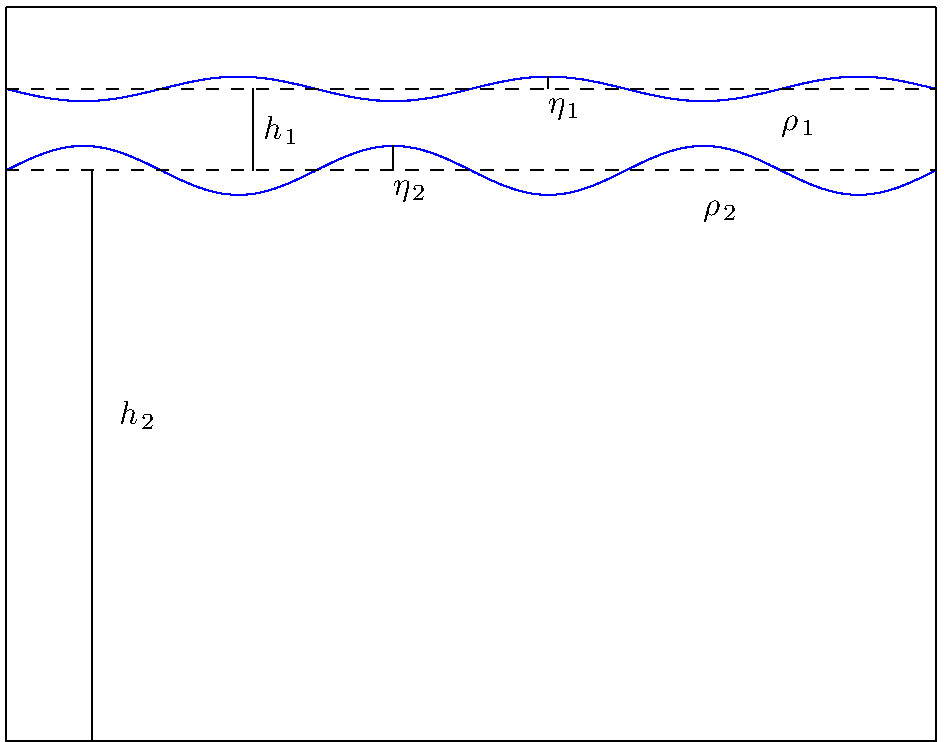
\includegraphics[height=3in]{Figures/two_layer_diagram.pdf}
\end{center}
\caption{Diagram of two layer system }
\label{twolayer}
 \end{figure}

The latter set of equations can be simplified by assuming a rigid lid approximation (no movement of free interface) and
assuming, without loss of generality, that the waves are propagating solely in the x direction.

% \begin{align}
%	u_{1t} - fv_1&= - g \eta_{1x}  \nonumber \\
%	v_{1t} + fu_1&= 0 \nonumber  \\
%	u_{2t} - fv_2&= - g' \eta_{2x} - g' \eta_{1x} \nonumber \\
%	v_{2t} + fu_2&= 0 \nonumber  \\
%	h_1 u_{1x} - \eta_{2t} &=0 \nonumber  \\
%	h_2 u_{2x} + \eta_{2t} &= 0
% \end{align}


 \begin{align}
	\dt{u_{1}} - fv_1&= - g \dx{\eta_{1}}  \nonumber \\
	\dt{v_{1}} + fu_1&= 0 \nonumber  \\
	\dt{u_{2}} - fv_2&= - g' \dx{\eta_{2}} - g' \dx{\eta_{1}} \nonumber \\
	\dt{v_{2}} + fu_2&= 0 \nonumber  \\
	u_2 &= - \frac{h_1}{h_2}u_1
 \end{align}

A plane wave solution of the following form is applied to the rigid-lid momentum equations. 

$$ (u_n, v_n, \eta_n) \sim (u_{no}, v_{no}, \eta_{no})e^{kx-\omega t}$$

where $k$ is the horizontal wave number, and $\omega$ is the angular frequency. Applying this solution to the two layer problem
yields the following dispersion relations. 

$$\omega_{BT}^2=f^2+gHk^2 $$
for the barotropic mode and
$$\omega_{BC}^2=f^2+g'\frac{h_1h_2}{H}k^2 $$
for the baroclinic mode (assuming a grid lid). 

The barotropic response corresponds to the two interfaces moving in phase with each other, as if the water body is homogenous. 
This response becomes important when the wavelength is comparable to the Rossby radius ($L_r=\frac{wave\ speed}{Coriolis\ frequency}=\frac{\sqrt{gH}}{f}$). 
For Lake Superior $L_r=400km$, much larger than the length of the basin and hence the barotropic response is not significant in 
the Lake Superior basin. 

The baroclinic response corresponds to the two interfaces moving out of phase with each other. This response becomes important
when the wavelength of a wave is comparable to the internal Rossby radius of deformation ($L_r=\frac{\sqrt{g'H'}}{f}$), which is on 
on the order of 4km for Lake Superior. Therefore, the baroclinic response is observable in the Lake Superior basin.  

%%%%%%%%%%%%%%%%%%%%%%%%%%%%
% POINCARE WAVES
%%%%%%%%%%%%%%%%%%%%%%%%%%%%
\section{Poincar\'{e} Waves}


When the wavelength of a wave is on the order of the Rossby radius of deformation then
the rotation of the earth starts to become important and the wave is classified as a Poincar\'{e} wave. 
Poincar\'{e} type waves are dispersive, the dispersion relation is : 


\begin{equation}
	\omega^2 = f^2 +gHk^2
\end{equation}

where $\omega$ is the frequency of the wave, $f$ is the Coriolis frequency, $g=9.8 ms^{-1}$ is gravitational acceleration, 
$H$ is the depth, and $k$ is the wavenumber.  The Coriolis frequency is given by $f=2\Omega \sin(\phi)$, where $\Omega=2*\pi day^{-1}$ 
is the rotation rate of the earth and and $\phi$ is the latitude. Duluth, MN sits at about 48$^{\circ}$ latitude and therefore 
$f=10^{-4}$ rad $s^{-1}$. An interesting feature of the dispersion relation is that the Coriolis frequency is
the lower limit of allowed frequencies. 

%When an internal wave has a period comparable to the period of Earth's rotation then
%the Coriolis force will be important. As a result of the Coriolis force, and hence the Earth's rotation, 
%the current vector will start to rotate around clockwise in the Northern hemisphere and counterclockwise
%in the southern hemisphere.  This is a force we must invoke because
%we are observing from a rotating platform (i.e. Earth). From our perspective, 
%the current vector for long internal gravity waves appears to rotate in around
%in a circle. Although it appears as though a force is changing the direction 
%of fluid flow, it is because we are on a moving platform. The mathematic treatment
%of this ficticious force was made by Coriolis and this invoked force hence has the
%name Coriolis force. The Coriolis force varies by latitude. The force is strongest 
%at the equator and gets weaker as you move toward either pole.  

\end{comment}

